\subsection{Concept Model of Knowledge Graph of Smart Home}
As shown in Figure~\ref{fig:conceptmodel}, concept model of knowledge graph is a knowledge abstraction of the concept level of smart home situational awareness service, describe the concept and the relationship between the abstract elements in the scenario of smart home.
\begin{figure}
	% \setlength{\belowcaptionskip}{0.1cm}
	\centering
	%	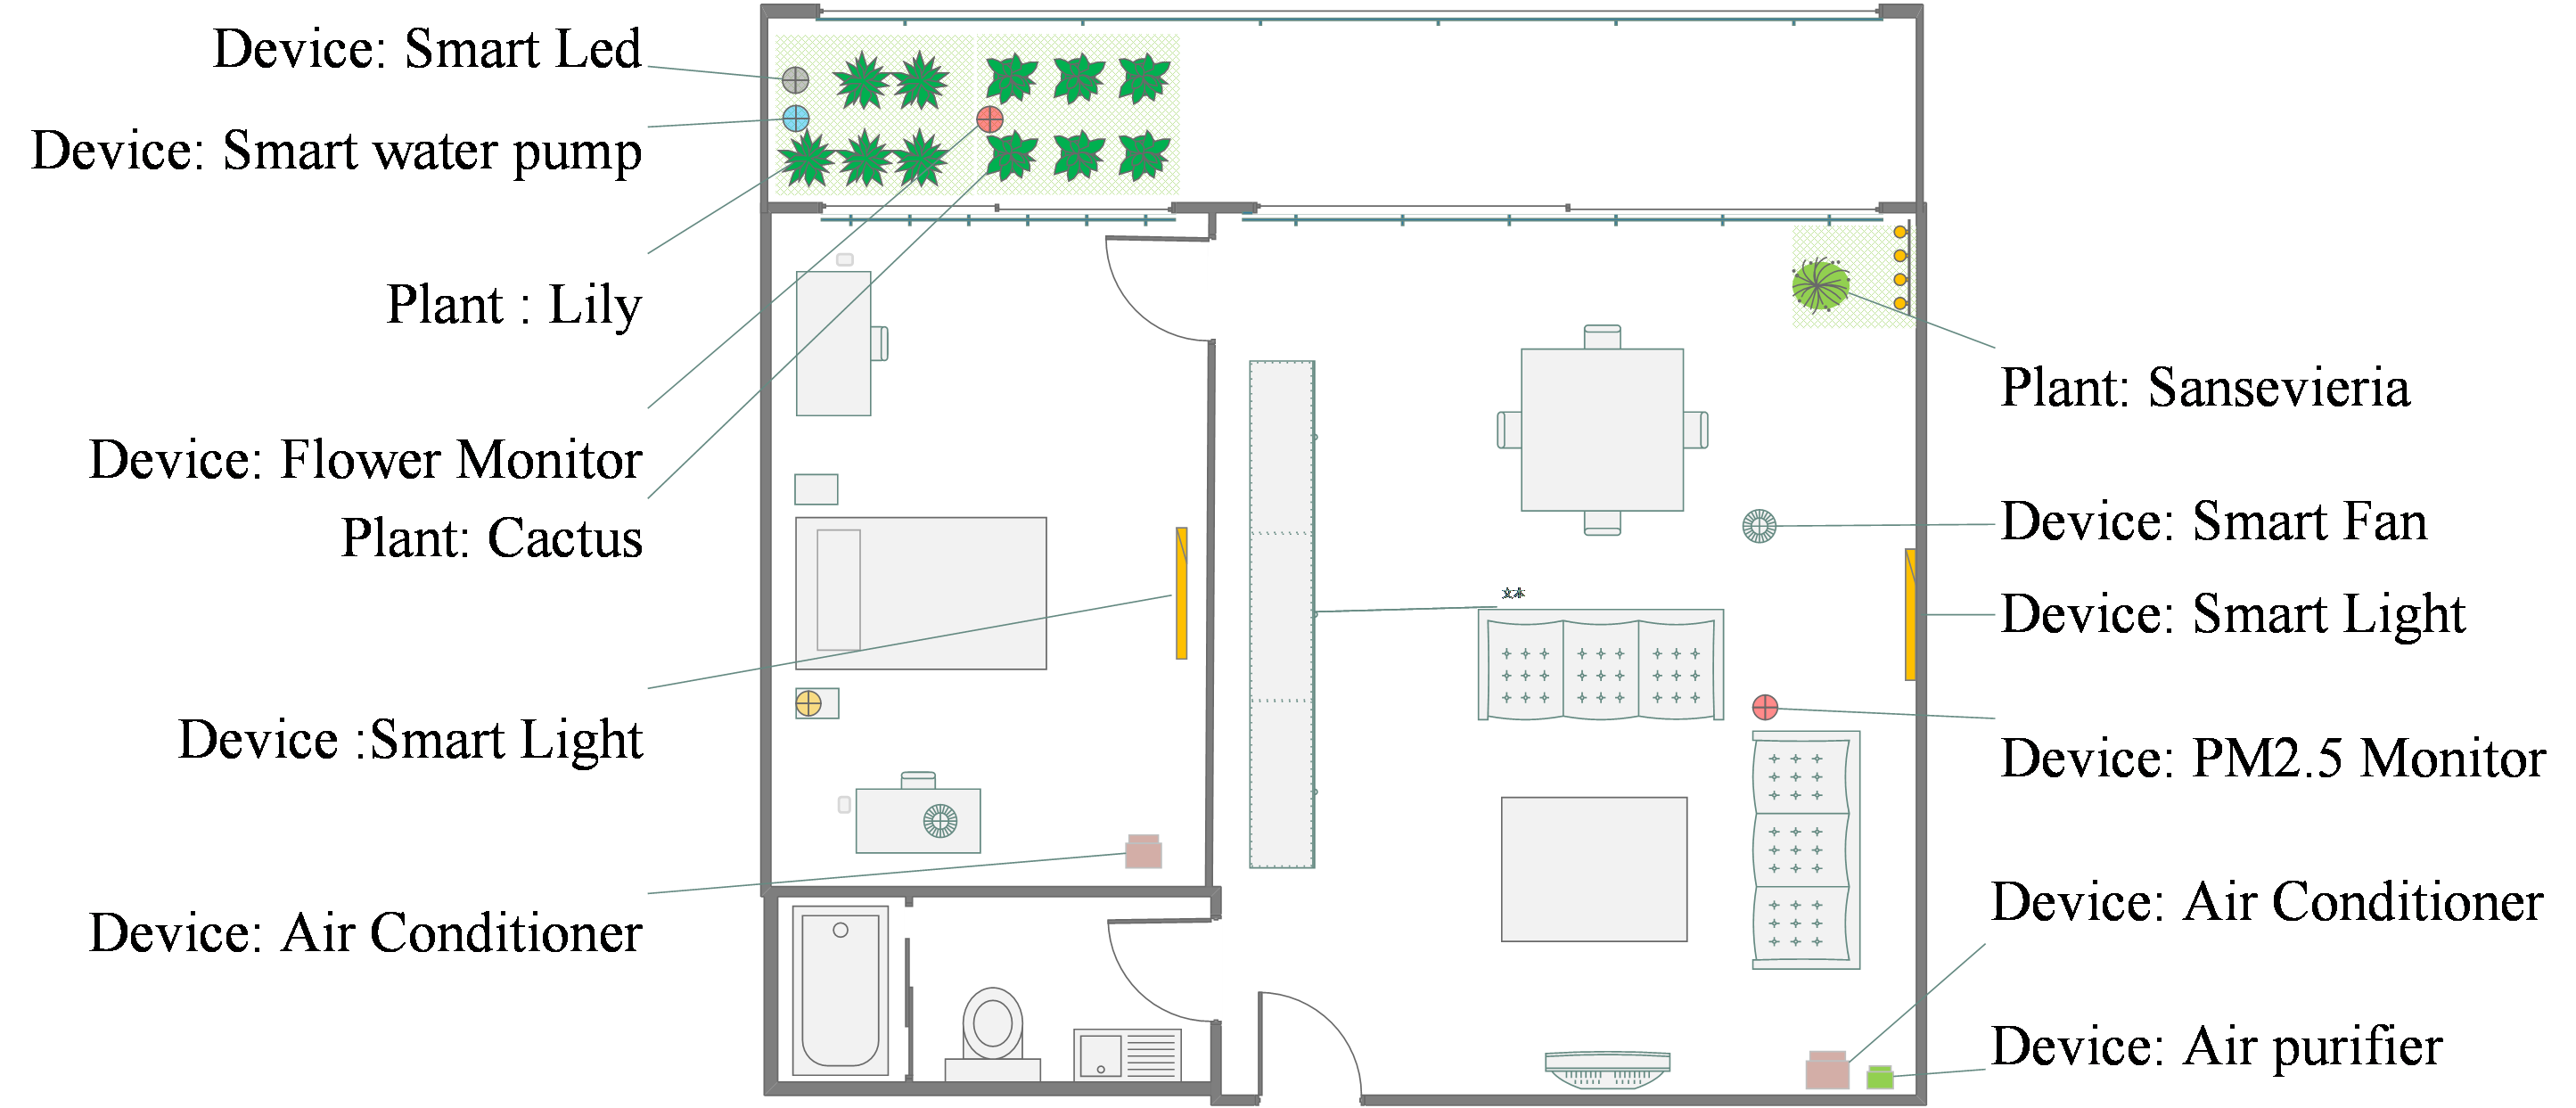
\includegraphics[width=0.9\textwidth]{Graph/scenario.png}
	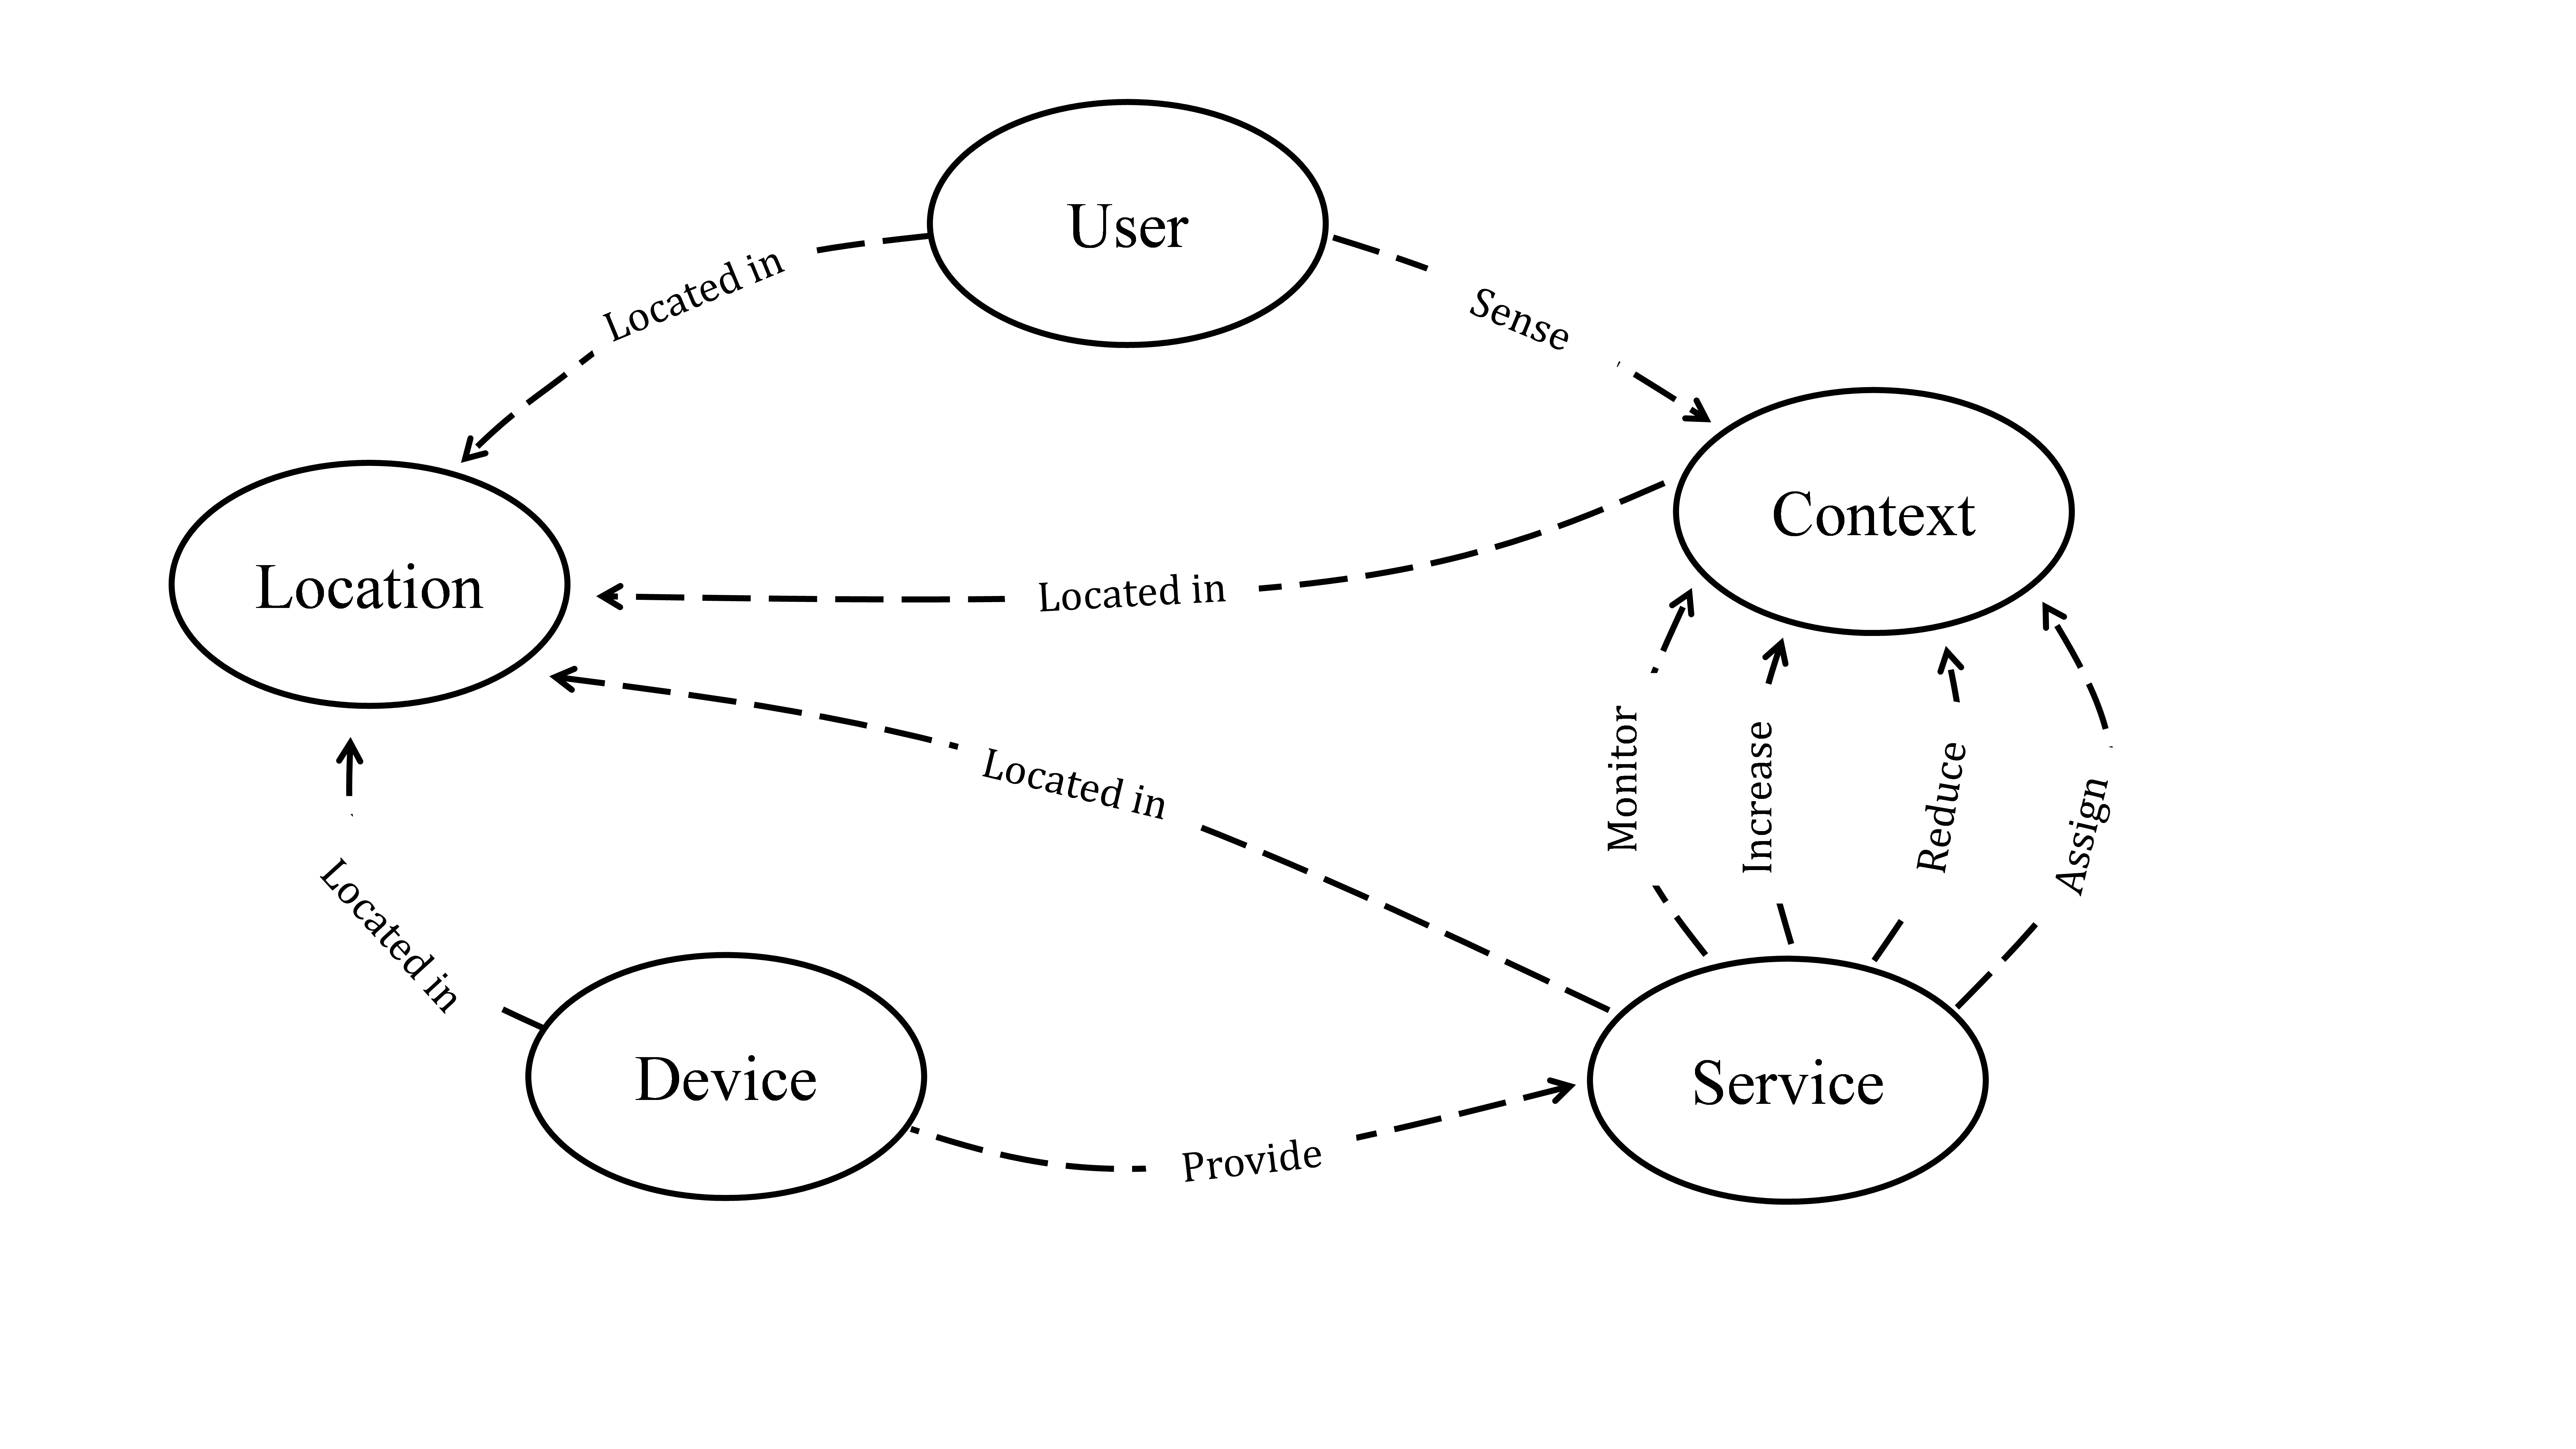
\includegraphics[width=0.9\textwidth]{conceptmodel.png}
	\caption{Concept Model of Knowledge Graph for Context-Aware Services of Smart Home}
	\label{fig:conceptmodel}
\end{figure}
The concept model defines the location, user, context, device, services and some concepts in the scenario of smart home, as shown in Table~\ref{table4}. Wherein, Location represents a specific area, the attribute LName represents the area name. User represents a service object, the attribute UName represents a user name, and the attribute LName represents a user's area. Context represents a certain environment state sensitive to the user. The attribute UName represents the user to which the environment state belongs, the attribute LName represents the area where the environment status is located, the attribute CType indicates the environment status type (for example, light, temperature, etc.). The attribute CValue represents the status value. The attributes RMin and RMax represent the range of state values that need to be met. Device represents a certain smart device. The attribute DName represents the device name. The attribute LName represents the area where the device is located. Status represents whether the device is enabled. The attribute Keyi represents the configuration parameter or system indicator of the device.Service represents a service provided by the smart device to monitor or change the state of the environment. The attribute DName represents the device providing the service, the attribute LName represents the area where the service is located, the attribute CType represents the environment status type of the service monitoring. The attribute Effect represents the effect on the state of the environment, mainly includes four types: Monitor, Increase, Reduce, and Assign. Status represents whether the service is enabled, and SValue represents the environmental status indicator (Monitoring) or service configuration parameters (Assignment).

\begin{table}[htbp]
	\caption{Concepts and Their Attributes in Concept Model of Knowledge Map for Smart Home}
	\centering  %表格居中
	\label{table4}  % 用于索引表格的标签
	\renewcommand\arraystretch{1.5}  %行高变为原来的1.5倍
	\begin{tabular}{|p{2cm}<{\centering}|p{8cm}|}  %指定列宽并居中
		\hline
		Concepts & Concept Attributes \\
		\hline
		Location & $<$ Lname $>$ \\
		\hline		
		User     & $<$ UName,LName $>$\\
		\hline		
		Context  & $<$ UName,LName,CType,CValue ,{RMin,RMax}$>$\\
		\hline		
		Device   & $<$ DName,LName, Status,{Key$_{1}$, Key$_{2}$,…, Key$_{n}$} $>$\\
		\hline		
		Service  & $<$ DName,LName,CType,Effect,Status,SValue $>$\\
		\hline	
	\end{tabular}
\end{table}
The concept model also defines the relationship such as Location in, Sense, Provide, Monitor, Increase, Reduce, Assign and so on , as shown in Figure~\ref{fig:conceptmodel}.

Among them, Located in  $X\xrightarrow[]{Located\,in}L$  represents User U,Context C,Device D,Service S and so on are located in Location L. Sense $U\xrightarrow[]{Sense}C$ represents User U perceives the state of Context C. Provide $D\xrightarrow[]{Provide}S$ represents that Device D provide Service S; Monitor $S\xrightarrow[]{Monitor}C$ represents that Service S is used to monitor the status value of Context C. Increase $S\xrightarrow[]{Increase}C$ represents that Service S is used to increase the state value of Context C. Reduce $S\xrightarrow[]{Reduce}C$ represents that Service S is used to lower the state value of Context C. Assign $S\xrightarrow[]{Assign}C$ represents that Service S is used to change the state value of Context C.

\subsection{Runtime modeling method of smart home knowledge graph instance model}

\subsubsection{Runtime modeling of conceptual instances}

\begin{table}[h]
	\caption{Mapping Rules for Model Operations of Location, User and Context Instances}
	\tiny
	\centering  %????
	\label{table1}  % ?????????
	\renewcommand\arraystretch{1.5}  %???????1.5?
	\newcommand{\tabincell}[2]{\begin{tabular}{@{}#1@{}}#2\end{tabular}}
	\begin{tabular}{p{0.5cm} p{3.6cm}<{\centering} p{3.6cm}<{\centering} p{3.6cm}<{\centering}}  %???????
		\toprule[1.5pt]
		& Location & User & Context \\
		\midrule[1.5pt]
		 List	&\tabincell{c}{List * L $\to$ \{L$_{1}$, L$_{2}$, ..., L$_{n}$\} \\  Get L$_{i}$.properties $\to$ L$_{i}$.properties} 
		 & \tabincell{c}{List * U $\to$ \{U$_{1}$, U$_{2}$, ..., U$_{n}$\} \\  Get U$_{i}$.properties $\to$ U$_{i}$.properties}  & \tabincell{c}{List * C $\to$ \{C$_{1}$, C$_{2}$, ..., C$_{n}$\} \\  Get C$_{i}$.properties $\to$ C$_{i}$.properties}  \\
		\midrule[1.5pt]
		
		 &  &  & Get C$_{i}$.UName $\to$ C$_{i}$.UName\\
		
		    &  &  & Get C$_{i}$.LName $\to$ Get U$_{j}$.LName(($\exists U_{j}$)($U_{j}\xrightarrow[]{Sense} C_{i}$))\\
		
		 Get  & Get L$_{i}$.LName $\to$ L$_{i}$.LName & Get U$_{i}$.UName $\to$ U$_{i}$.UName  & Get C$_{i}$.CType $\to$ C$_{i}$.CType\\
		
		    &  & Get U$_{i}$.LName $\to$ \textbf{RTModel} (Get $T_{i}$.location) & Get C$_{i}$.CValue $\to$ Get S$_{j}$.SValue(($\exists S_{j}$)($S_{j}\xrightarrow[]{Monitor}C_{i}$)$\bigwedge$($S_{j}.Status="On")$))\\
			&  &  & Get C$_{i}$.RMin $\to$ C$_{i}$.RMin \\
			&  &  & Get C$_{i}$.RMax $\to$ C$_{i}$.RMax \\
		\midrule[1.5pt]
			Set       & - & - & -\\
		\bottomrule[1.5pt]
	\end{tabular}
\end{table}

\begin{table}[h]
	
	\tiny
	\centering  %????
	\label{table1}  % ?????????
	\renewcommand\arraystretch{1.5}  %???????1.5?
	\newcommand{\tabincell}[2]{\begin{tabular}{@{}#1@{}}#2\end{tabular}}
	\begin{tabular}{p{0.5cm} p{4.5cm}<{\centering} p{4.5cm}<{\centering} }  %???????
		\toprule[1.5pt]
		& Device & Service  \\
		\midrule[1.5pt]
		List	& \tabincell{c}{List * D $\to$ \{D$_{1}$, D$_{2}$, ..., D$_{n}$\} \\  Get D$_{i}$.properties $\to$ D$_{i}$.properties}  & \tabincell{c}{List * S $\to$ \{S$_{1}$, S$_{2}$, ..., S$_{n}$\} \\  Get S$_{i}$.properties $\to$ S$_{i}$.properties} \\
		\midrule[1.5pt]
		
		&  &   Get S$_{i}$.DName $\to$ S$_{i}$.DName\\%1
		
		& Get D$_{i}$.DName$\to$ D$_{i}$.DName & Get S$_{i}$.LName $\to$ Get D$_{j}$.LName(($\exists D_{j}$)($D_{j}\xrightarrow[]{Provide} S_{i}$))\\%2
		
	   Get & Get D$_{i}$.LName$\to$ D$_{i}$.LName &   Get S$_{i}$.CType $\to$ S$_{i}$.CType \\%3
	    & Get D$_{i}$.Key$_{m}$ $\to$ \textbf{RTModel} (Get D$_{i}$.Key$_{m}$) &   Get S$_{i}$.Effect $\to$ S$_{i}$.Effect \\%4
	    &  &   Get S$_{i}$.Status $\to$ Get D$_{j}$.Key$_{m}$(($\exists D_{j}$)($D_{j}\xrightarrow[]{Provide} S_{i}$))\\%5
	    &  &   Get S$_{i}$.SValue $\to$ Get D$_{j}$.Key$_{n}$(($\exists D_{j}$)($D_{j}\xrightarrow[]{Provide} S_{i}$))\\%6
	   \midrule[1.5pt]
		Set       & Set D$_{i}$.Key$_{m}$ $\to$ \textbf{RTModel} (Set D$_{i}$.Key$_{m}$) & Set S$_{i}$.Status $\to$ Set D$_{j}$.Key$_{m}$(($\exists D_{j}$)($D_{j}\xrightarrow[]{Provide} S_{i}$))\\
				  &  & Set S$_{i}$.SValue $\to$ Set D$_{j}$.Key$_{n}$(($\exists D_{j}$)($D_{j}\xrightarrow[]{Provide} S_{i}$) $\bigwedge$ ($S_{i}.Effect="Assign"$))\\
		\bottomrule[1.5pt]
	\end{tabular}
\end{table}

\paragraph{}
The knowledge graph concept model defines the concepts in the smart home scenes such as location, user, context, device and service. The concept instances are constructed based on the configuration of developers. The two-way synchronization between the concept instance attributes and the scene real-time information is realized through model operation transformation.



Related configurations provided by the developer include scenario-oriented situational knowledge, mapping relationship between concept instances and smart devices, constraints on the context in which the service objects are located, and descriptions of specific locations, users, contexts, devices, and services in the scenario.The scenario-oriented context knowledge provides a set of locations \{L$_{1}$, L$_{2}$, ..., L$_{n}$\} in a specific scenario. The mapping relationship between the concept instance and the smart device provides the device set \{D$_{1}$, D$_{2}$, ..., D$_{n}$ \} in the specific scenario. It provides a set of services \{S$_{1}$, S$_{2}$, ..., S$_{n}$\}, and the relationship between the device and the service; the constraints of the context in which the service object is located describe the set of users \{U$_{1}$, U$_{2}$, ..., U$_{n}$\} in the specific scenario, set of its positioning devices \{T$_{1}$, T$_{2}$, ..., T$_{n}$\}, and the user-sensitive set of environmental states \{C$_{1}$, C$_{2}$,..., C$_{n}$\}.Then, according to the location set L, the user set U, the context set C, the device set D and the service set S, a concept instance of the corresponding type is constructed. Meanwhile, the SM@RT tool[7, 8] is used to construct the smart device and the positioning device. We use runtime model to manage the smart device and positioning device at the model level[9].

The model operation of the concept instance mainly includes three types, namely List, Get, and Set. Among them, “List” represents listing all instances of concept of the type and its attributes, “Get” represents getting the attribute value of concept instance, and “Set” represents setting the attribute value of concept instance. In order to maintain the two-way synchronization of the knowledge map concept instance attribute and the scene real-time information, we define the model operation conversion rule of the concept instance, as shown in Table 5. The location instance L$_{i}$, the value of the attribute LName is from the configuration. User instance U$_{i}$, the value of its attribute UName comes from the configuration.Its attribute LName, which is consistent with the attribute LName of the corresponding device T$_{i}$ in the positioning device runtime model, and the value of the T$_{i}$ is automatically read when the value of the U$_{i}$ attribute LName is read. That is Get U$_{i}$.LName $\to$ \textbf{RTModel} (Get $T_{i}$.location).The context instance C$_{i}$, whose values of the attributes UName and CType are from the configuration. Its attribute LName corresponds to the LName of user instance $U_{j} (U_{j}\xrightarrow[]{Sense} C_{i})$. The value of the U$_{j}$ attribute LName is automatically read when the value of the C$_{i}$ attribute LName is read, that is Get C$_{i}$.LName $\to$ Get U$_{j}$.LName(($\exists U_{j}$)($U_{j}\xrightarrow[]{Sense} C_{i}$)).CValue of context instance is same as the SValue of corresponding service instance $S_{j}\xrightarrow[]{Monitor}C_{i}$.The value of the S$_{j}$ attribute SValue is automatically read when the value of the C$_{i}$ attribute CValue is read, that is Get C$_{i}$.CValue $\to$ Get S$_{j}$.SValue(($\exists S_{j}$)($S_{j}\xrightarrow[]{Monitor}C_{i}$)). Its properties RMin and RMax are from configuration. The attributes DName and LName of the device instance D$_{i}$ are from the configuration. Its attribute Key$_{m}$, which is the same as the attribute Key$_{m}$ of the corresponding D$_{i}$ in the smart device runtime model. When reading/writing the Key$_{m}$ of D$_{i}$ , it will automatically read/write the Key$_{m}$ of D$_{i}$ in the runtime model. That is Get D$_{i}$.Key$_{m}$ $\to$ \textbf{RTModel} (Get D$_{i}$.Key$_{m}$) / Set D$_{i}$.Key$_{m}$ $\to$ \textbf{RTModel} (Set D$_{i}$.Key$_{m}$) .Service instance S$_{i}$, the values of its attributes DName, CType, and Effect, from configuration . The LName of Service instance is the same as the SValue of corresponding device instance. The value of the D$_{j}$ attribute LName is automatically read when the value of the S$_{i}$ attribute LName is read, that is Get S$_{i}$.LName $\to$ Get D$_{j}$.LName(($\exists D_{j}$)($D_{j}\xrightarrow[]{Provide} S_{i}$)). The attribute Status is consistent with the attribute Key$_{m}$ of the device instance D$_{j}$ indicating whether the device is enabled or not. And the value of the D$_{i}$ attribute Key$_{m}$ is automatically read/written when the Status is read/written. That is Get S$_{i}$.Status $\to$ Get D$_{j}$.Key$_{m}$ / Set S$_{i}$.Status $\to$ Set D$_{j}$.Key$_{m}$(($\exists D_{j}$)($D_{j}\xrightarrow[]{Provide} S_{i}$)). The attribute SValue is consistent with the attribute Key$_{n}$ indicating the corresponding environment state in the corresponding device instance D$_{j}$, and the value of the D$_{i}$ attribute Key$_{n}$ is automatically read/written when the value of the S$_{i}$ attribute SValue is read/written. That is Get S$_{i}$.SValue $\to$ Get D$_{j}$.Key$_{n}$ / Set S$_{i}$.SValue $\to$ Set D$_{j}$.Key$_{n}$(($\exists D_{j}$)($D_{j}\xrightarrow[]{Provide} S_{i}$))




\subsubsection{Runtime modeling of relational instances}
\paragraph{}
The knowledge graph conceptual model defines the relationship between concepts in smart home scenarios such as location,  provision, monitoring, improvement, reduction, and assignment, and further defines the runtime construction rules of the relationship instance, as shown in Table 6. When two concept instances satisfy certain preconditions, the relationship instance between them is constructed. Among them, there are instances $X_{i}$ and location instance $L_{j}$ of the user, environment, device, service, etc., and the value of the $X_{i}$ attribute LName is the same as the value of the $L_{j}$ attribute LName. Construct a relationship instance $X_{i}\xrightarrow[]{Located\,in}L_{j}$, indicating that the concept instance $X_{i}$ is located in the location instance $L_{j}$. The relationship instance $U_{i}\xrightarrow[]{Sense} C_{j}$, indicating that the user instance $U_{i}$ senses the environment instance $C_{j}$, the relationship instance $D_{i}\xrightarrow[]{Provide}S_{j}$, indicating that the device instance $D_{i}$ provides the service instance $S_{j}$, both from the configuration information. The service instance $S_{i}$ and the environment instance $C_{j}$ exist, the values of the $S_{i}$ attributes LName, CType and the $C_{j}$ attributes LName, CType are the same, and the $S_{i}$ attribute When the value of Effect is Monitor, the relationship instance $S_{i}\xrightarrow[]{Monitor}C_{j}$ is constructed, indicating that the service instance $S_{i}$ is used to monitor the state value of the environment instance $C_{j}$. The service instance $S_{i}$ and the environment instance exist. $C_{j}$, the value of the $S_{i}$ attribute LName, CType is the same as the value of the $C_{j}$ attribute LName, CType, and the value of the $S_{i}$ attribute Effect is Increase, the relationship instance $S_{i}\xrightarrow[]{Increase}C_{j}$ is constructed, indicating that the service instance $S_{i}$ is used to improve the environment. The state value of the instance $C_{j}$. The existence of the service instance $S_{i}$ and the environment instance $C_{j}$, the values of the $S_{i}$ attributes LName, CType and the values of the $C_{j}$ attributes LName, CType are the same, and the value of the $S_{i}$ attribute Effect is Reduce, constructing the relationship instance $S_{i}\xrightarrow[]{Reduce}C_{j}$, indicating that the service instance $S_{i}$ is used to reduce the state value of the environment instance $C_{j}$. There is a service instance $S_{i}$ and an environment instance $C_{j}$, the values of the $S_{i}$ attributes LName, CType are the same as the values of the $C_{j}$ attributes LName, CType, and the $S_{i}$ attribute Effect When the value is Assign, the relationship instance $S_{i}\xrightarrow[]{Assign}C_{j}$ is constructed, indicating that the service instance $S_{i}$ is used to change the state value of the environment instance $C_{j}$. In addition, since the concept instance attribute is kept in two-way synchronization with the scene real-time information, the relationship instance will be Change as its attribute value changes.

\begin{table}[htbp]
	\caption{Rules for Constructing Relation Instances}
	\centering  %表格居中
	\label{table5}  % 用于索引表格的标签
	\renewcommand\arraystretch{1.5}  %行高变为原来的1.5倍
	\begin{tabular}{|c|c|}  %指定列宽并居中
		\hline
		Relationship instance & Precondition \\
		\hline
		$X_{i}\xrightarrow[]{Located\,in}L_{j}$ & $X_{i}.LName$=$L_{j}.LName$ \\
		\hline		
		$U_{i}\xrightarrow[]{Sense} C_{j}$      & - \\
		\hline		
		$D_{i}\xrightarrow[]{Provide}S_{j}$     & - \\
		\hline		
		$S_{i}\xrightarrow[]{Monitor}C_{j}$     & $S_{i}.LName=C_{j}.LName$ $\Lambda$ $S_{i}.CType=C_{j}.CType$ $\Lambda$ $S_{i}.Effect$ =``Monitor"\\
		\hline		
		$S_{i}\xrightarrow[]{Increase}C_{j}$    & $S_{i}.LName=C_{j}.LName$ $\Lambda$ $S_{i}.CType=C_{j}.CType$ $\Lambda$ $S_{i}.Effect$ =``Increase"\\
		\hline	
		$S_{i}\xrightarrow[]{Reduce}C_{j}$      & $S_{i}.LName=C_{j}.LName$ $\Lambda$ $S_{i}.CType=C_{j}.CType$ $\Lambda$ $S_{i}.Effect$ =``Reduce"\\
		\hline
		$S_{i}\xrightarrow[]{Assign}C_{j}$      & $S_{i}.LName=C_{j}.LName$ $\Lambda$ $S_{i}.CType=C_{j}.CType$ $\Lambda$ $S_{i}.Effect$ =``Assign"\\
		\hline
	\end{tabular}
\end{table}

\subsubsection{Status update for the instance model}
\paragraph{}
In order to maintain the two-way synchronization of the smart home knowledge map instance model and the scene real-time information, the instance model automatically updates the state:

1. Update the concept instance, which in turn is a location instance, a user instance, a device instance, a service instance, and an environment instance.

2. Update the relationship instance, which in turn is the ``Located in" instance, the ``Monitor" instance, the ``Increase" instance, the ``Reduce" instance, and the ``Assign" instance.

3. Repeat execution 1.

\subsection{Knowledge Graph Concept Model Modeling Example}

According to the knowledge of the smart home scenario mentioned above, combined with the example of the smart home scenario in Chapter 2, construct the knowledge graph instance model. According to the example of the smart home scenario in Chapter 2, there are three location instances, corresponding to three regions in the scenario. This section takes some parts of the living room as an example, as shown in Figure~\ref{fig:ch4}.
%\begin{figure}
%	% \setlength{\belowcaptionskip}{0.1cm}
%	\centering
%	%	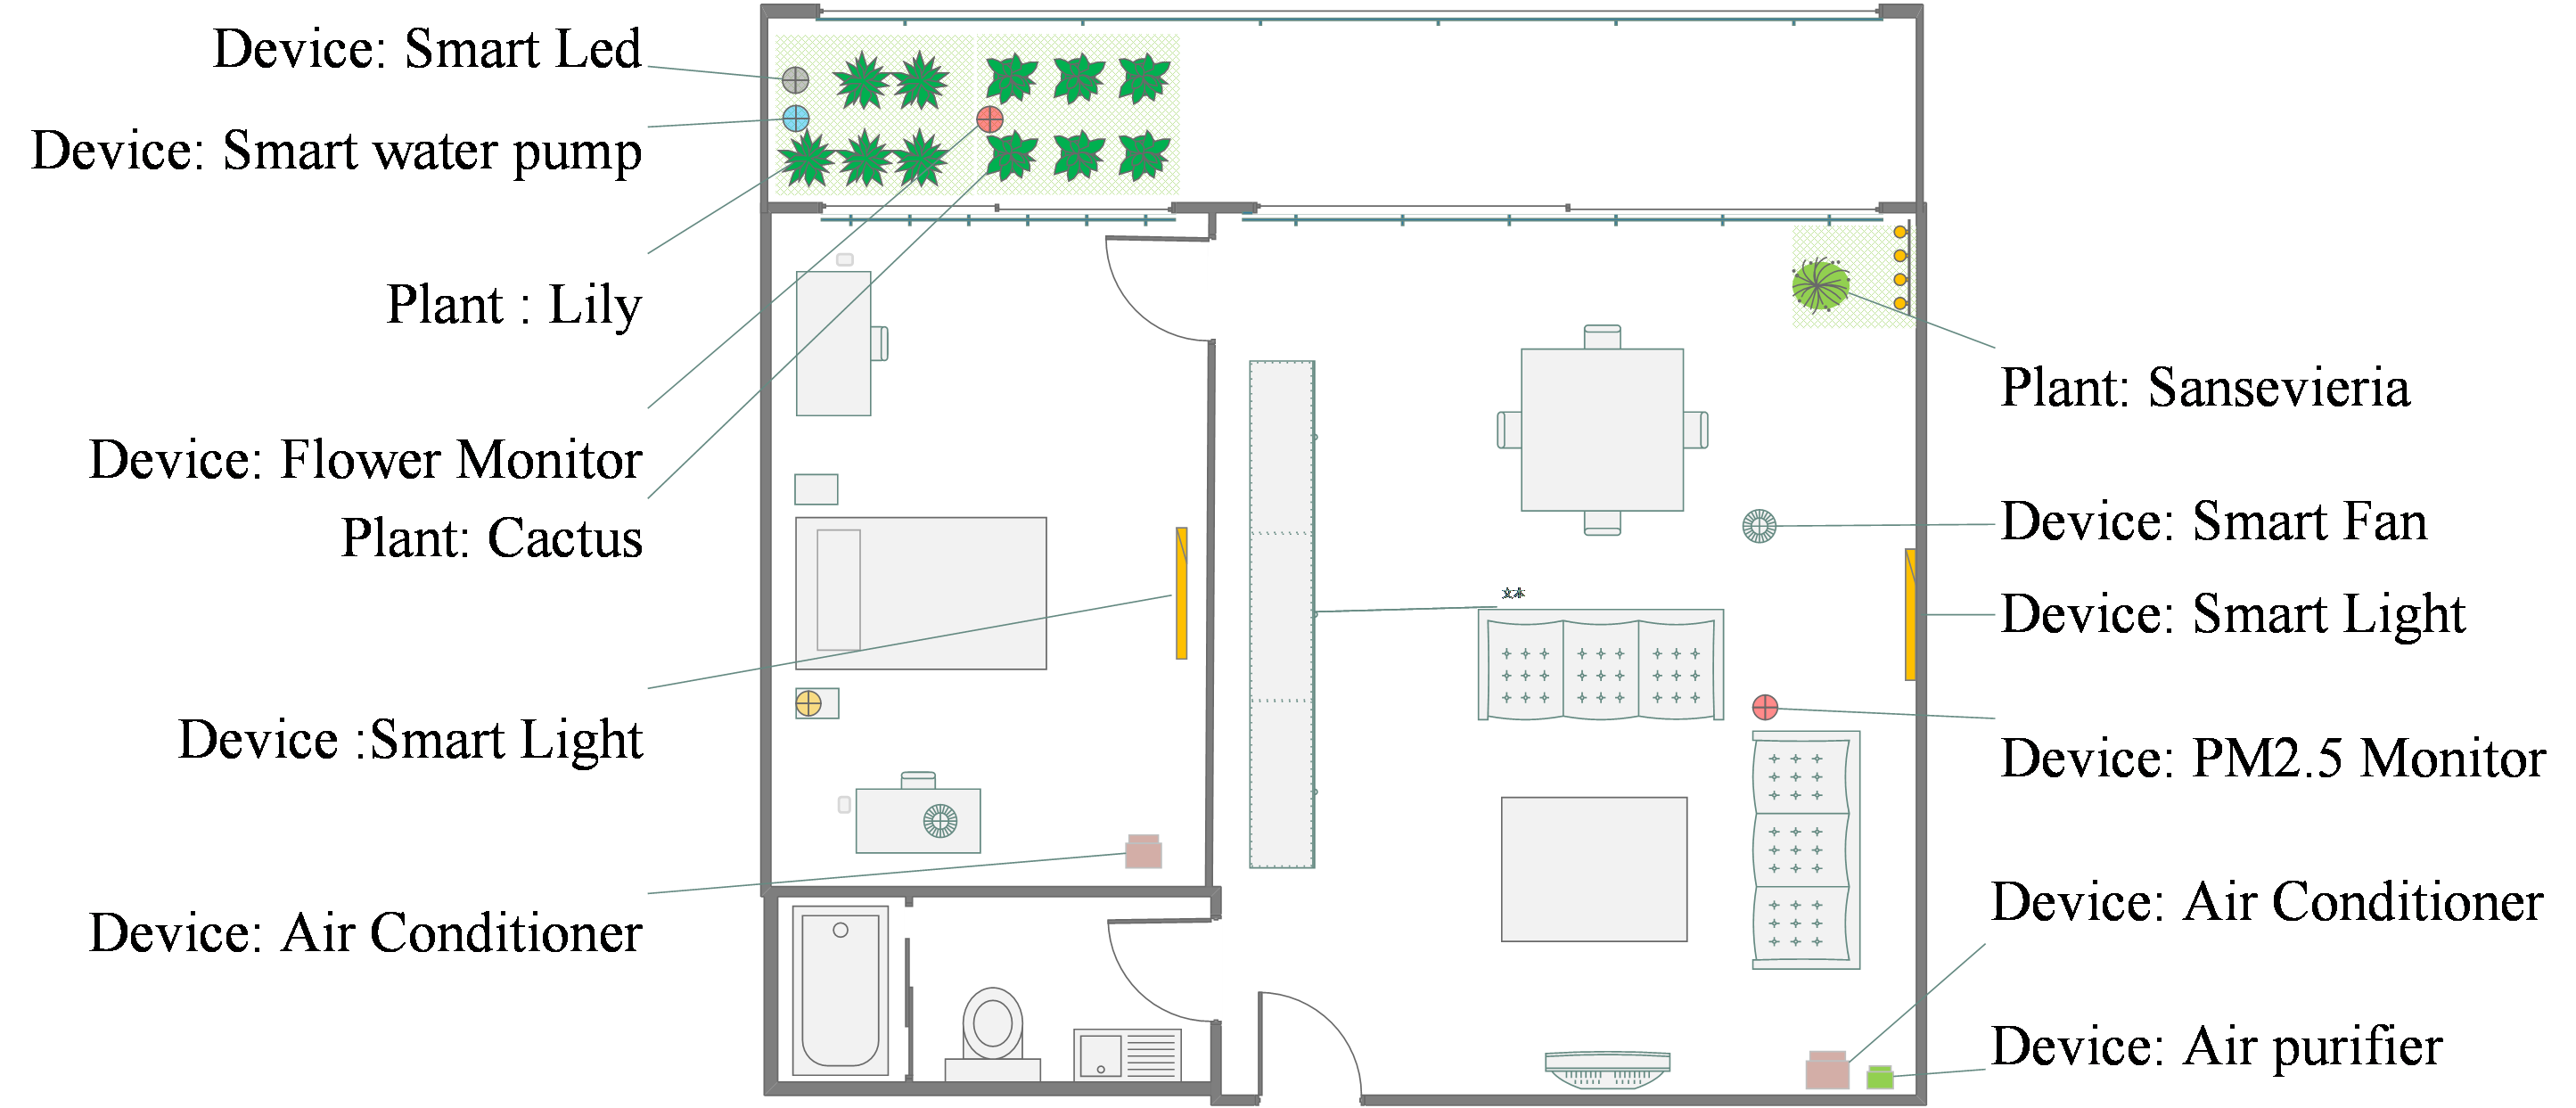
\includegraphics[width=0.9\textwidth]{Graph/scenario.png}
%	\includegraphics[width=0.9\textwidth]{ch4.png}
%	\caption{Instance Model of the Knowledge Graph for Smart Home}
%	\label{fig:ch4}
%\end{figure}
According to the knowledge of the smart home scenario mentioned above, combined with the example of the smart home scenario in Chapter 2, construct the knowledge graph instance model. According to the example of the smart home scenario in Chapter 2, there are three location instances, corresponding to three regions in the scenario. This section takes some parts of the living room as an example, as shown in Figure 4.
There are two user instances in the living room, which correspond to two service objects in the scene. $U_{1}$ corresponds to Jack, and its attribute LName indicates the area where it is consistent with the corresponding element attribute retention value in the positioning device runtime model. $U_{2}$ corresponds to sansevieria. There are three environment instances, which correspond to the sensitive environment status of each service object in the scenario. For example, the sensitive environment state of Jack ($U_{1}$) is in the same state as the attribute LName of $U_{1}$, and the environment status type is temperature, state value and The attribute SValue of the corresponding service instance maintains the same value, and the constraint range of the state value is [19$^{\circ}$C, 26 $^{\circ}$C]. There are three device instances, which correspond to the Air-Conditioning, Smart Light, and PM2.5 Monitor in the scene. For example, the PM2.5 detector located in the living room has the attribute LName indicating the area, and its attributes $On\_Off$ and PM2.5 are respectively related to the attributes $On\_Off$ and PM2.5 of the corresponding PM2.5 detector device in the smart device runtime model. Consistent. There are 8 service instances, which correspond to the services provided by the smart devices in the scenario; for example, the smart light tube located in the living room has the same value of the LName and the attribute LName of the smart light tube device, and the environmental status type is light intensity. (Brightness), the service type is Monitor, Increse, Assign, whose attribute Status is consistent with the attribute $On\_Off$ of the corresponding device instance, and the attribute SValue and the attribute Brightness of the corresponding device instance are maintained. Consistent.
